% --------------------------------------------------------
%                   请用Xelatex编译
%                   请用Xelatex编译
%                   请用Xelatex编译
%                   请用Xelatex编译
%                   请用Xelatex编译
% --------------------------------------------------------
\documentclass[UTF8,12pt]{ctexart}

\usepackage[a4paper,left=2.5cm,right=2.5cm,top=2.5cm,bottom=2.5cm]{geometry}    % 这个包专门用来调整页边距
\usepackage{amsmath}    % 数学包
\usepackage{fancyhdr}   % 页眉页脚设定

% 插入图片的包
\usepackage{graphicx}
\usepackage{subfigure}

% 插入表格的包
\usepackage{float}
\usepackage{booktabs}
\usepackage{multirow}

% 删去图注、表注的冒号
\usepackage{caption}
\DeclareCaptionLabelSeparator{twospace}{\ ~}   %%这三条语句即可
\captionsetup{labelsep=twospace}

% 颜色包,定义颜色,会在附录中使用到
\usepackage{xcolor}
\definecolor{gray}{RGB}{128,128,128}

% 链接包:这个宏包在论文中没有任何作用,单纯为了方便给我做广告
% 让目录可以索引到正文,所以这个包不能删!
\usepackage{hyperref}
\hypersetup{colorlinks=true,linkcolor=black,citecolor=blue,filecolor=black,urlcolor=cyan,pdftitle={Overleaf Example},pdfpagemode=FullScreen}
    
% 附录插入代码
\usepackage{listings}
\lstset{basicstyle=\ttfamily,columns=fullflexible,frame=single,breaklines=true,keywordstyle=\color{blue},commentstyle=\color{gray}}

% 务必注意:图片在figures目录下
% 务必注意:图片在figures目录下
% 务必注意:图片在figures目录下
\graphicspath{{figures/}} 



\begin{document}   % 文章开始



% ----------------------------------------------- %
%              请在这里输入文章标题
% ----------------------------------------------- %
%              请在这里输入文章标题
% ----------------------------------------------- %
\title{基于树的影响因素预判与信息挖掘}



\author{} % 不要动!!
\date{} % 不要动!!
\maketitle % 不要动!!
\vspace{-4em}  % 不要动!!



% ---------------------------------------------------- %
%  打开chapter文件夹里的摘要.tex文件,编辑其中的内容
% ---------------------------------------------------- %
%  打开chapter文件夹里的摘要.tex文件,编辑其中的内容
% ---------------------------------------------------- %
\begin{abstract}

    摘要是全文最重要的部分,也是阅卷人首先看到的部分,阅卷人会只根据摘要将文章分成三六九等,所以如果不认真写摘要的话你就会有大麻烦,请务必留至少两小时用于摘要的打磨,将其控制在1面!!!
    
    针对问题一:在写摘要的时候请搞清楚,首先摘要的第一段是题设的背景,你需要随便胡扯几句,但别扯太多,毕竟要把摘要控制在一面很难!然后写完第一段后从第二段开始就要开始介绍你对每个题目的理解、过程以及求解与评价,语言尽量精炼,不要啰嗦,再强调一次:那么多内容的摘要压缩在一面非常难!下面我将给大家演示如何对于自己已经完成的“模型建立与求解”部分进行摘要描述。
    
    针对问题二,本文基于可视化和假设检验对所给数据集进行数据分析。首先对产品的销售价格和销售量的关系进行探究,本文分别通过\textbf{斯皮尔曼相关系数}对相关性进行定量描述,求得$\rho$=-0.2946,反映出\textbf{销售价格和销售量的相关性较弱}。接着对区域与销量的关系进行探究,通过\textbf{方差检验}得知\textbf{不同地区对订单的需求量有显著差异},并通过直方图探究出不同区域产品的需求量的不同特性。然后,本文对产品的销售方式与需求量的关系进行探究,通过\textbf{Mann-Whitney U}检验得出\textbf{线上销售与线下销售的销售量存在显著差异}。最后,通过\textbf{单样本Wilcoxon符号秩检验}将时间序列整体与促销活动单日的销量相比较,得出\textbf{促销活动单日的销量与平时的销量有显著差异}。为了将各特征的分布以及定量分析所得出的结论直观化,本文利用小提琴图、箱线图、直方图等对相关特征进行可视化,结果与定量分析一致。
    
    针对问题三,摘要内容摘要内容摘要内容摘要内容摘要内容摘要内容摘要内容摘要内容摘要内容摘要内容摘要内容摘要内容摘要内容摘要内容摘要内容摘要内容摘要内容摘要内容摘要内容摘要内容摘要内容摘要内容摘要内容摘要内容摘要内容摘要内容摘要内容摘要内容摘要内容摘要内容摘要内容摘要内容摘要内容摘要内容摘要内容摘要内容摘要内容摘要内容摘要内容摘要内容摘要内容摘要内容摘要内容摘要内容摘要内容摘要内容摘要内容摘要内容摘要内容摘要内容摘要内容摘要内容摘要内容摘要内容摘要内容摘要内容摘要内容。
    
    第二部分分别是针对数据分析的任务和机器学习的任务,可以看到摘要第一句话用于概括整个小题大致是怎么做的,从第二句话开始展开每一步,用“首先”、“接着”、“然后”、“最后”依次描述。在摘要中务必要把你的结果和评价情况直接呈现出来并且加粗,同时你使用的关键方法也需要加粗,通过这个源文件相信你已经知道该如何加粗了。
    
    \vspace{1em} % 移除2个行距的空白:这句代码千万不能动!!!移除2个行距的空白:这句代码千万不能动!!!
    
    \noindent{\textbf{关键词:}随机森林;方差选择法;Voting Classifier;层次聚类分析;决策树}
    
\end{abstract} 



\thispagestyle{empty}  % 清除摘要页的页码,不要动!!
\newpage  % 另开一页写目录,不要动!!



% ------------------------------------------------------------ %
%    这一部分自动生成目录,同时清除目录页的页眉和页脚,
%    清除目录页的页码以保证正文的第一面为页码1
%    并新开一面,如果不想要目录直接删除这部分
% ------------------------------------------------------------ %
\pagestyle{fancy}
\fancyhead{} % 页眉清空
\fancyfoot{} % 页脚清空
\begin{center} \tableofcontents \end{center} 
\thispagestyle{empty}\newpage



% ------------------------------------------------------------ %
%    设置正文的页眉、页脚,页眉没有内容,页码在页脚中间
%    并将本页设置为第一页
%    我浅浅用页眉给自己做了个广告,大家记得删除啊!
% ------------------------------------------------------------ %
\pagestyle{fancy} % 不要动!!
% 这是个广告,正式使用时请删除这一行
% 删除上一行后将下面的这句\fancyhead[R]{}前面的百分号删除就行
\fancyhead[R]{}
\fancyhead[C]{} % 页眉中间清空 不要动!!
\fancyhead[L]{} % 页眉左侧清空 不要动!!
\fancyfoot[R]{} % 页脚右侧清空 不要动!!
\fancyfoot[C]{- {\thepage}\ -} % 页脚中间为页码 不要动!!
\fancyfoot[L]{} % 页脚左侧清空 不要动!!
\setcounter{page}{1}  % 不要动!!



% ---------------------------------------------------------- %
% 接下来的部分即为文章每个章节的内容,我这里使用的是2022年
% 国赛的论文,当时是有四道题目,每次竞赛的题目量都不一定,
% 请酌情更改,另外有时候可能会多一个灵敏度分析或是其他创新
% 的内容,记住一个准则:有多少个章节就在chapter文件夹中制作
% 多少个tex文件,每个文件夹管一个章节就行啦!!!
% ---------------------------------------------------------- %



% ---------------------------------------------------------- %
%    打开chapter文件夹里的问题重述.tex文件,编辑其中的内容
% ---------------------------------------------------------- %
%    打开chapter文件夹里的问题重述.tex文件,编辑其中的内容
% ---------------------------------------------------------- %
\section{问题重述}

\subsection{问题背景}

数学建模比赛论文是要我们解决一道给定的问题,所以正文部分一般应从问题重述开始,一般确定选题后就可以开始写这一部分了。
这部分的内容是将原问题进行整理,将问题背景和题目分开陈述即可,所以基本没啥难度。
本部分的目的是要吸引读者读下去,所以文字不可冗长,内容选择不要过于分散、琐碎,措辞要精练。
注意:在写这部分的内容时,绝对不可照抄原题!(论文会查重)
应为:在仔细理解了问题的基础上\cite{ref1},用自己的语言重新将问题描述一遍。语言需要简明扼要,没有必要像原题一样面面俱到。


\subsection{问题提出}

看到上面插入的“\cite{ref1}”了吗,这是在引用后面的文献,所以大家在文中引用文献的时候也像我这样在句子结束后面加一个这个就行了,他是蓝色的,比较醒目,一般也都是蓝色的好像。

现有一组由专家给出的关于玻璃的数据,要求通过分析与建模解决下面若干问题:

\textbf{问题1:} 问题提出内容问题提出内容问题提出内容问题提出内容问题提出内容问题提出内容问题提出内容问题提出内容。

\textbf{问题2:} 问题提出内容问题提出内容问题提出内容问题提出内容问题提出内容问题提出内容问题提出内容问题提出内容问题提出内容。

\textbf{问题3:} 问题提出内容问题提出内容问题提出内容问题提出内容问题提出内容问题提出内容问题提出内容问题提出内容问题提出内容。

\textbf{问题4:} 问题提出内容问题提出内容问题提出内容问题提出内容问题提出内容问题提出内容问题提出内容问题提出内容问题提出内容。



% ---------------------------------------------------------- %
%    打开chapter文件夹里的问题分析.tex文件,编辑其中的内容
% ---------------------------------------------------------- %
%    打开chapter文件夹里的问题分析.tex文件,编辑其中的内容
% ---------------------------------------------------------- %
\section{问题分析}

本文对于赛题题设,从多个角度对数据集进行统计分析与统计推断,本部分将对四个问题进行简要分析,同时赛题的每个问题的解答完整流程以流程图的形式在附录A给出。

\subsection{问题一的分析}

针对问题一,第一问要求关于术中、术后 24h 不良反应,判断新药组和原有药物组是否存在显著差异。首先对附件1中进行数据清洗、特征缩放、特征编码,由于不良反应在编码后均为分类特征,故用基于多变量可视化分析的定性方法和基于卡方检验的定量方法探究不同药组对于不良反应的差异性。

第二问要求建立一个有效的分类模型用于对患者的不良反应进行预判。本文基于经过数据预处理的数据集,首先对标签进行分布分析,并对标签比例严重失衡的数据集进行上采样处理。接着把数据按比例分为训练集和测试集。然后基于决策树对训练集进行特征提取,使用经过训练的决策树模型实现对两大类、8组不良反应的预判。最后基于混淆矩阵、ROC图对模型在测试集上的表现进行评价。


\subsection{问题二的分析}

针对问题二,第一问要求判断新药组和原有药物组在生命体征数据方面是否表现出显著差异。首先对数据进行数据清洗和特征编码。接着基于Spearman、Kendall相关性分析计算特征之间的相关性并删除相关性高特征之一,为避免高维数据集造成数据分析困难,基于主成分分析法在保留较高方差解释比例的前提下对数据进行降维。最后对降维后的特征进行正态性检验,分别基于独立样本t检验和Mann-Whitney U研究不同药组对生命体征数据的差异性。

第二问在第一问的基础上,探究造成新药对生命体征数据显著差异的影响因素。本文基于经过数据预处理的数据集,基于LightGBM对以受试者情况和病史为特征空间、以检验出显著差异的生命特征组为标签的数据集进行特征提取,在确保模型性能极好的前提下并利用树模型独有的特征重要性评价功能对各特征对标签的作用效果进行评价,最后利用条形统计图呈现。

\subsection{问题三的分析}

针对问题三,要求根据用药信息和患者信息预测对给药后 3 分钟以内的 IPI 数据。首先对数据进行数据清洗和特征编码。接着为了避免大量分类特征造成特征空间离散从而影响模型提取特征,基于主成分分析法对特征空间进行降维。然后基于岭回归和支持向量机回归分别对数据集进行特征提取,并用线性加权法对二者结果进行融合。最后为了提高模型的可靠性和准确性,本文基于MAE、MSE和数据扰动对模型在测试集上的表现和回归的稳定性进行评价。


\subsection{问题四的分析}

针对问题四,要求基于现有数据找出与术后满意度有关的因素,本文使用定性方法和定量方法分别进行模型求解。

基于斯皮尔曼、肯德尔相关性分析分别对数值特征和分类特征与术后满意度的相关性进行探究。首先对数据进行数据清洗,对分类特征进行特征编码,对数值特征进行特征缩放。接着对两类特征分别进行相关性分析,求得相关系数。最后用条形统计图对结果进行可视化,得出初步结论。

基于树模型的树状图对术后满意度划分的定量探究。首先对数据进行预处理,并将五维关于术后满意度的特征聚合为一维关于术后满意度的评分作为标签,为避免术后满意度评分分布不均衡导致模型难以提取特征,对数据集进行上采样。然后按比例将数据集划分为训练集和测试集,并基于随机森林对训练集进行特征提取。最后导出随机森林的树状图,并通过树状图获取分类的具体依据。


















% ---------------------------------------------------------- %
%    打开chapter文件夹里的模型假设.tex文件,编辑其中的内容
% ---------------------------------------------------------- %
%    打开chapter文件夹里的模型假设.tex文件,编辑其中的内容
% ---------------------------------------------------------- %
\section{模型假设}

% 这个地方开始涉及到顺序环境,也就是1,2,3……排序,每个序号一个\item,然后用\begin{enumerate}和\end{enumerate}包起来就可以

\begin{enumerate}
  \item 假设本文的数据真实可靠。
  \item 假设患者除了使用本题所用药物外,未使用其他药物。
  \item 假设患者出现的不良反应是除了环境等客观因素造成的。
  \item 本文认为所给的数据不存在过大的人为过失。
  \item 假设患者在用药前并未吃其他食物。
  \item 本文认为药物在存放过程中成分没有发生改变。
\end{enumerate} 



% ---------------------------------------------------------- %
%    打开chapter文件夹里的符号说明.tex文件,编辑其中的内容
% ---------------------------------------------------------- %
%    打开chapter文件夹里的符号说明.tex文件,编辑其中的内容
% ---------------------------------------------------------- %
\section{符号说明}

% 这里涉及到表格插入的问题,这里真的不太好描述,大家自己摸索吧,很简单。
% 然后提醒一下,如果使用表注,将会依次计入序号,如果不使用就不计入序号
% 也就是说:第一个使用表注的表是表1,而不是第一个出现的表


\begin{table}[H]
	\centering  % 不要动!
	\begin{tabular}{c c}  % 有几列就要有几个c,c与c之间用空格
		\toprule[1.5pt]  % 不要动!
		符号 & 含义  \\   % 列与列之间用  & 隔开,下同
		\midrule[1pt]    % 不要动!
        ${{\chi }^{2}}$	            &  卡方检验的卡方值  \\
        ${{O}_{ij}}$                &  第$i$个样本的第$j$种特征存在数量  \\
        ${{E}_{ij}}$                &  第$i$个样本的第$j$种特征不存在数量  \\
        $df$	                    &  特征的自由度  \\
        $p$	                        &  样本的p值  \\
        $\chi$                      &  特征空间  \\
        ${{\overrightarrow{x}}_{i}}$ &	第$i$个样本的特征向量  \\
        ${{L}_{3}}\left( \cdot  \right)$ & 计算闵可夫斯基距离  \\
        ${{c}_{j}}$	 &  第$j$个分类指标  \\
        ${{d}_{i}}$	 &  第$i$个样本的等级  \\
        $H(\overrightarrow{x})$  &  组合模预测型向量函数  \\
        $erro{{r}_{ij}}$	     &  第$i$个特征的第$j$个样本扰动值  \\
		\toprule[1.5pt]  % 不要动!
	\end{tabular}  
\end{table} 











% ------------------------------------------------------------ %
%    打开chapter文件夹里的问题一建模.tex文件,编辑其中的内容
% ------------------------------------------------------------ %
%    打开chapter文件夹里的问题一建模.tex文件,编辑其中的内容
% ------------------------------------------------------------ %
\section{问题一的模型建立与求解}

%\subsection{数据预处理}

\subsection{模型建立}

模型建立部分是需要有大量的数学公式的,而很多小伙伴都没有 \LaTeX 基础,这里就不得不提到Mathtype了,队友可以先用Mathtype在Word或者WPS中敲好公式,然后再用Mathtype直接将公式转换为Tex代码。Mathtype安装、配置方法可以在我的个人网页中找到哈,仅供学习使用,不可用作商业用途!

值得注意的是这样转换而来的代码还是需要修改的,但是这个修改很容易!!!首先要注意,转换出来的代码全都是用:

\begin{lstlisting}
\[数学公式Tex代码\]
\end{lstlisting}

当然不排除我的Mathtype版本不对,正版、新版的已经修正。如果这样的话你需要把行内公式改为用一前一后的一对“\$”包裹,而行间公式则是用专门的数学环境——equation环境包裹。行内公式和行间公式示例如下:

\begin{lstlisting}
% Mathtype转化出的行内数学公式Tex代码
本部分使用\[\dfrac{4}{5}\]的数据集作为训练集……

% 正确修改为
本部分使用$\dfrac{4}{5}$的数据集作为训练集……
\end{lstlisting}

\begin{lstlisting}
% Mathtype转化出的行间数学公式Tex代码
即可得到:
\[a+b\leq c+d\]

% 正确修改为
即可得到:
\begin{equation}
    a+b\leq c+d
\end{equation}
\end{lstlisting}





\subsection{模型求解}



% ------------------------------------------------------------ %
%    打开chapter文件夹里的问题二建模.tex文件,编辑其中的内容
% ------------------------------------------------------------ %
%    打开chapter文件夹里的问题二建模.tex文件,编辑其中的内容
% ------------------------------------------------------------ %
\section{问题二建模与求解}

%\subsection{数据预处理}

\subsection{模型建立}

\subsection{模型求解}



% ------------------------------------------------------------ %
%    打开chapter文件夹里的问题三建模.tex文件,编辑其中的内容
% ------------------------------------------------------------ %
%    打开chapter文件夹里的问题三建模.tex文件,编辑其中的内容
% ------------------------------------------------------------ %
\section{问题三的建模与求解}

%\subsection{数据预处理}

\subsection{模型建立}

\subsection{模型求解}



\section{问题四的建模与求解}

\subsection{相关性分析}

为了找出与术后满意度相关的特征,我们将以术后满意度为标签来计算各个特征的相关性,使用Spearman和Kendall相关性分析,Spearman相关系数公式已给出,介绍Kendall原理:

设有两个随机变量$\overrightarrow{X}=\left( {{x}_{1}},{{x}_{2}},...,{{x}_{n}} \right),\overrightarrow{Y}=\left( {{y}_{1}},{{y}_{2}},...,{{y}_{n}} \right)$,将它们分别排名得到两个的排名向量$\overrightarrow{X}=\left( {{r}_{1}},{{r}_{2}},...,r \right),\overrightarrow{Y}=\left( {{s}_{1}},{{s}_{2}},...,{{s}_{n}} \right)$,得到相关系数:

\begin{equation}
    \tau = \dfrac{2}{n(n-2)}\sum_{i=1}^{n-1}\sum_{j=i+1}^{n}\text{sgn}{(x_i-x_j)}\text{sgn}{(y_i-y_j)}.
\end{equation}
其中,表示$\text{sgn}(x)$的$x$符号系数,当$x>0$时,$\text{sgn}(x)=1$,当$x=0$时,$\text{sgn}(x)=0$,当$x<0$时,$\text{sgn}(x)=-1$。分别计算得到的相关性如下图所示:

\begin{figure}[H] % 这个H不要动!
	\centering % 不要动!
	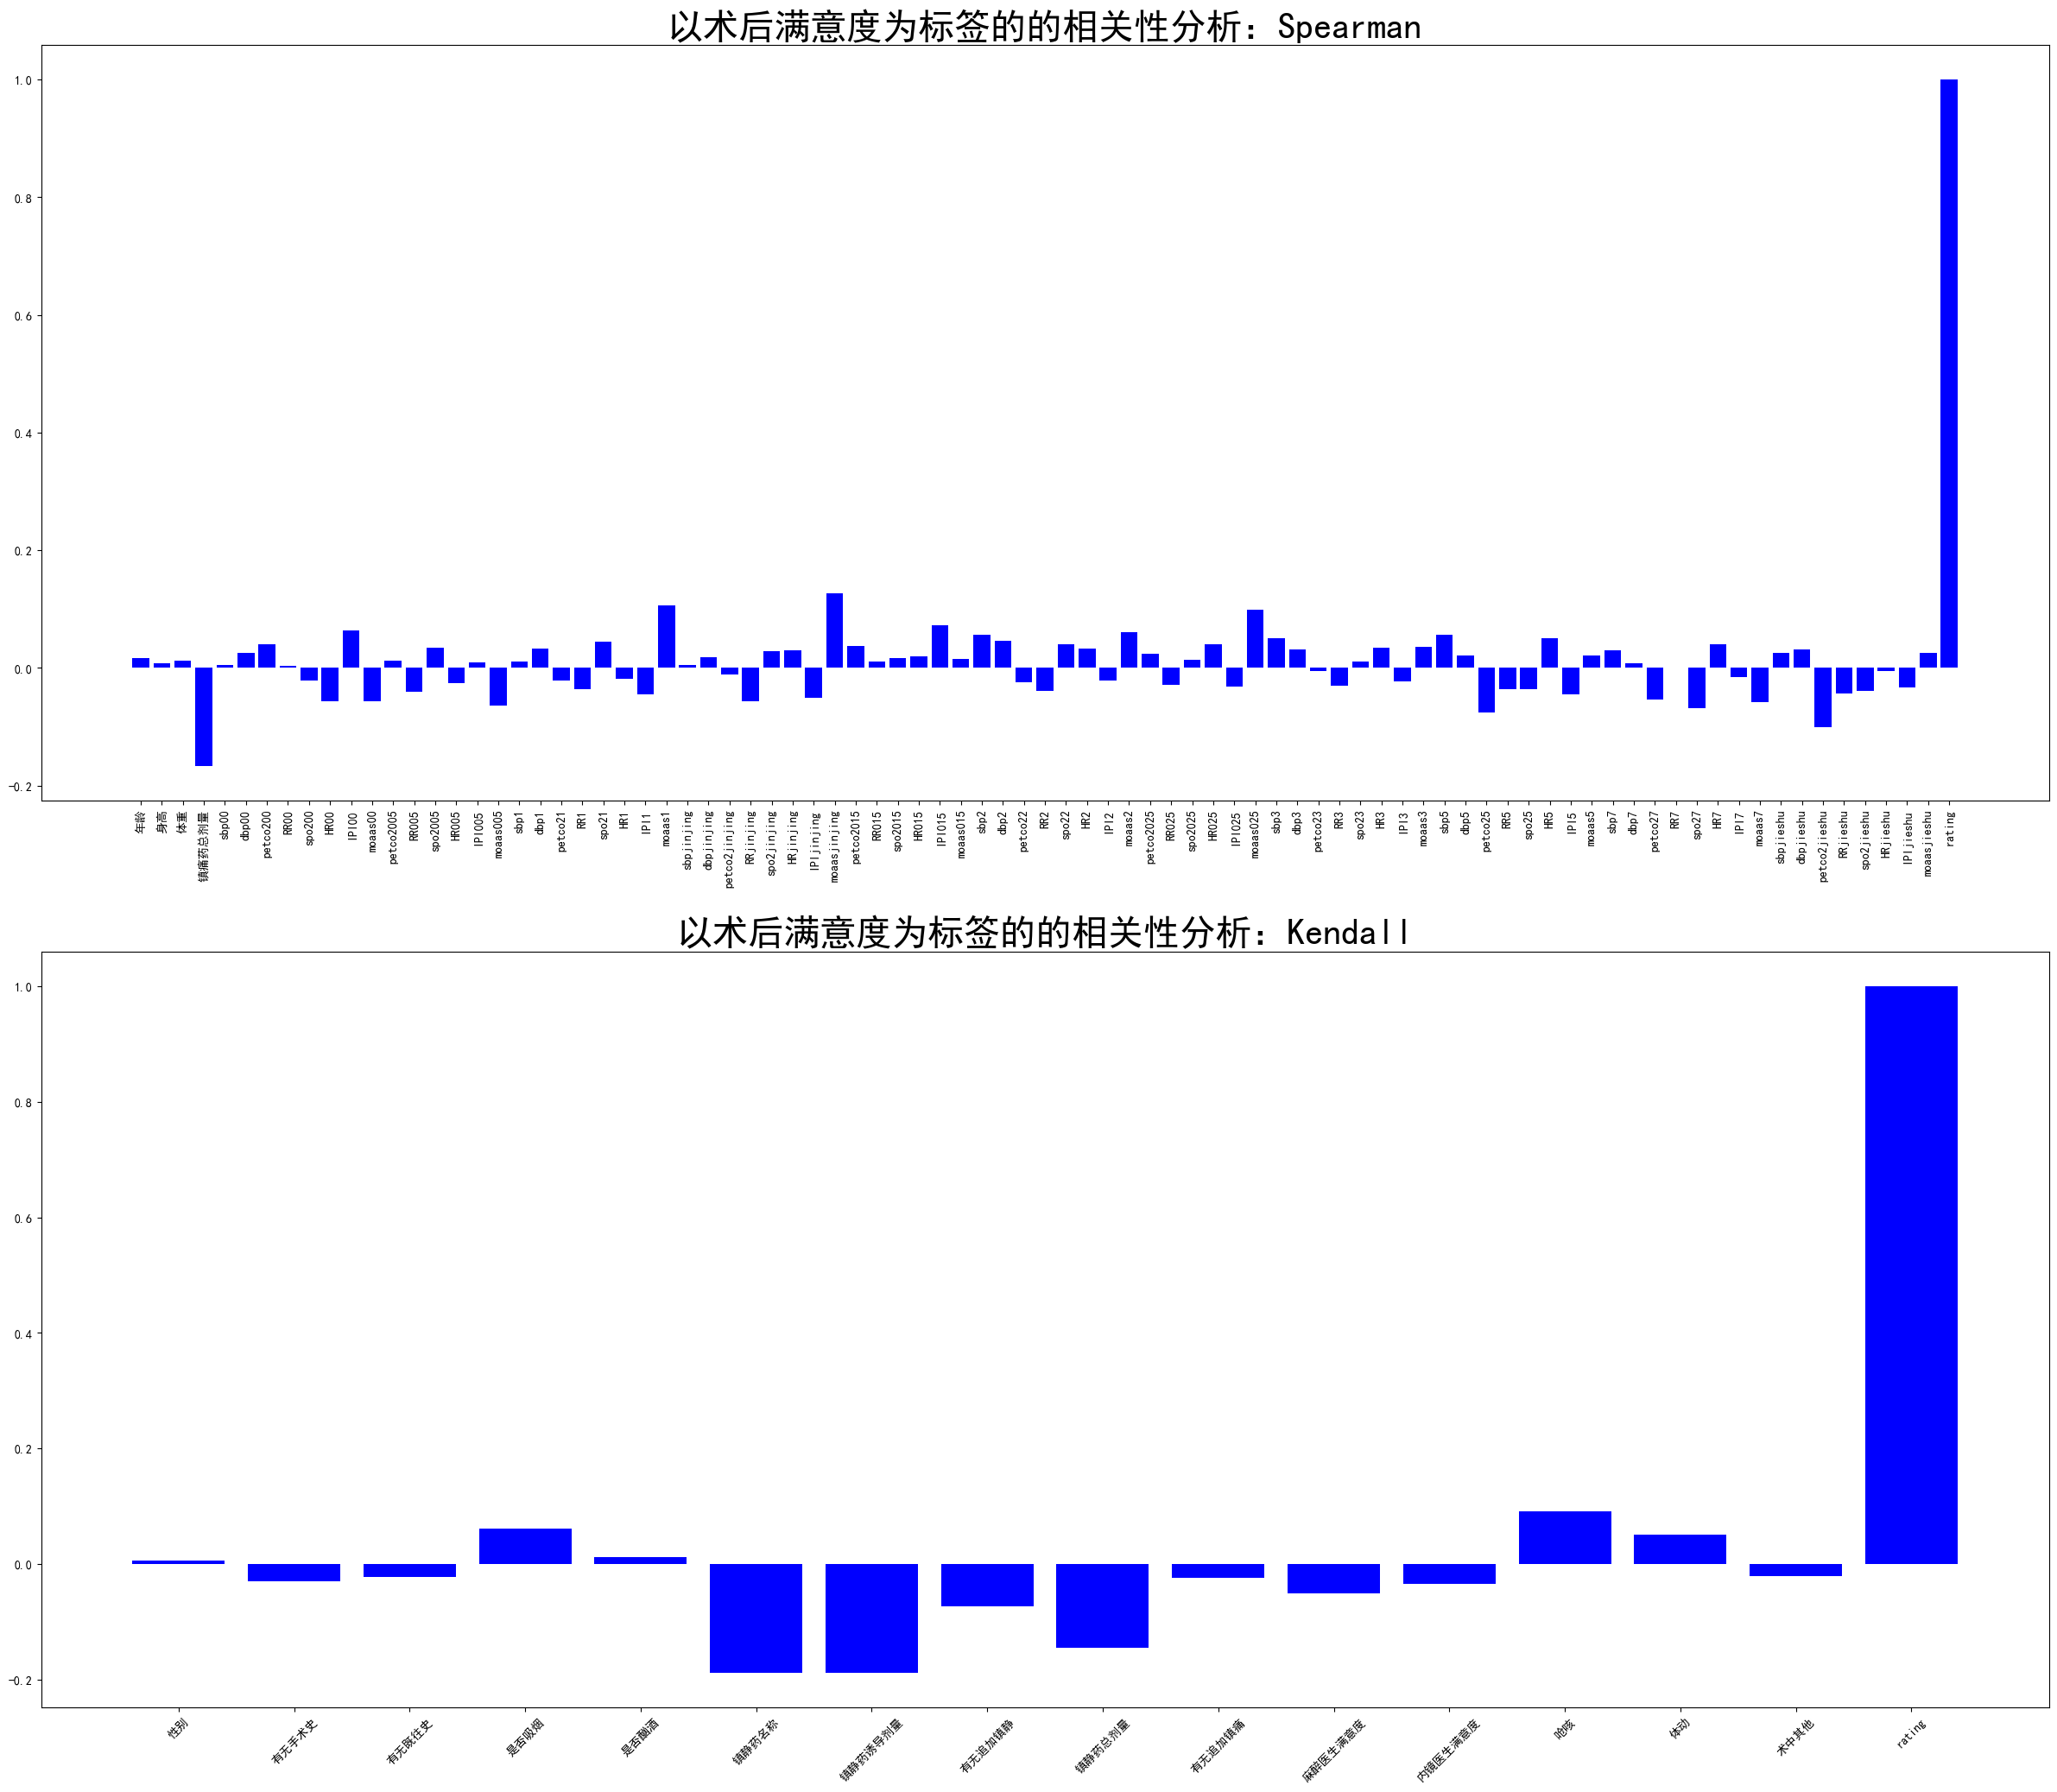
\includegraphics[width=0.95\textwidth]{10.png} 
	\label{Fig.main10} 
    \caption{以术后满意度为标签的相关性分析}
\end{figure}


由上图可知,第一个图展示的是使用Spearman相关性分析得到的各个特征与标签之间的相关系数,而第二个图展示的是使用Kendall方法得到的相关系数,条形图的x轴是各个特征的名称,y轴则是相应的相关系数。分析上图,由上分图关于数值型特征与术后满意度的Spearman相关系数得到相关性分析可以看出镇痛药的总剂量对于术后满意度的不良影响最大,这与现实情况是吻合的。而moaasjinjing与术后满意度的正向影响相关性最大,其中关于moaas的含量与术后满意的都有正相关性的关系,综合考虑,相关性的绝对值都不大于0.2。从统计学上分析存在的相关性并不大,但是相对而言镇痛药的对术后满意度的不良影响的相关性较大。由第二张图关于分类特征与术后满意度的Kendall相关性分析可以看出镇静药名称、镇静药诱导剂量、镇静药总剂量对于术后满意度的不良影响最大,而其他因素对于术后满意度的正向影响相关性都比较弱,综合考虑,相关性的绝对值都不大于0.2。从统计学上分析存在的相关性并不大,但是相对而言镇静药的名称、镇静药诱导剂量、镇静药总剂量对术后满意度的不良影响的相关性较大。综上,镇痛药和镇静药各种因素对于术后满意程度都有不利的影响,而moaas的含量对于术后满意度的影响是有利的。


通过这个图可以直观地比较不同特征与标签之间的相关性强度,但是由于术后满意度标签分布不均衡,可能会影响模型提取特征的效果,进而影响其准确率和稳定性,需要进一步优化模型。


\subsection{基于随机森林的分类标准挖掘}

为进一步探究出与术后满意度有关的因素,并挖掘出其间的定量关系,本文基于随机森林算法建立模型

\subsubsection{模型建立}

随机森林是一种集成学习方法,由多棵决策树组成。其公式可以分为两部分:随机森林的生成和随机森林的预测。随机森林的生成过程如下:

\begin{enumerate}
  \item 从原始数据集中采样出$n$个样本作为训练集,采用 bootstrap 技术进行采样,即每次从原始数据集中随机抽取一个样本并将其放回,重复$n$次得到大小为$n$的采样集。
  \item 从所有特征中随机选择$m$个特征,其中$m\ll d$,$d$为原始特征的总数。
  \item 利用上述采样得到的数据集和特征集构建一棵决策树,具体建树过程可以使用 ID3、C4.5 或 CART 等决策树算法。
  \item 重复步骤前三步$T$次,得到$T$棵决策树,这些决策树构成了随机森林。
\end{enumerate}
  
  
随机森林的预测步骤:

\begin{enumerate}
  \item 对于每个测试样本,对随机森林中的每棵决策树进行预测,得到预测结果。
  \item 对$T$个预测结果进行投票,将得票最多的类别作为随机森林的最终预测结果。
\end{enumerate}

随机森林的预测公式可以表示为:

\begin{equation}
    \widehat{y}=\arg {{\max }_{y}}\sum\limits_{i=1}^{T}{I\left( {{\widehat{y}}_{i}}=y \right)}.
\end{equation}
其中,$\widehat{y}$表示随机森林的预测结果,${{\widehat{y}}_{i}}$表示第$i$棵决策树的预测结果,$T$表示随机森林中的决策树数量,$y$表示所有可能的类别,$I(\cdot )$表示指示函数,当条件成立时取值为1,否则取值为 0。




\subsubsection{模型求解}

通过对标签进行分布分析,得出如下条形统计图:

\begin{figure}[H] % 这个H不要动!
	\centering % 不要动!
	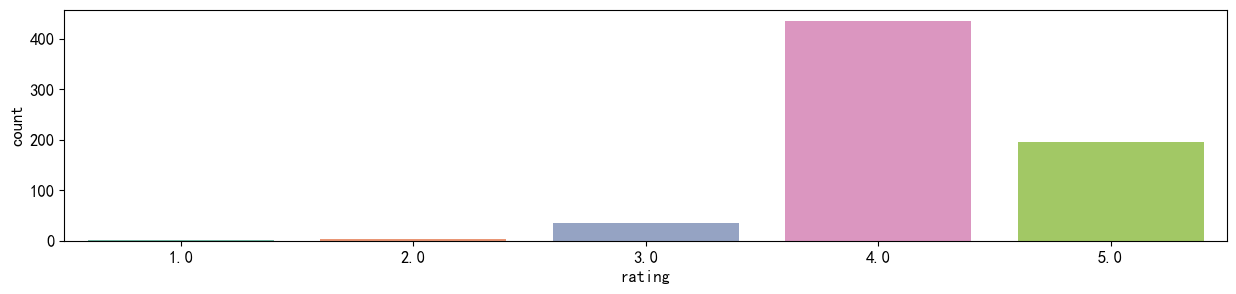
\includegraphics[width=0.95\textwidth]{11.png} 
	\label{Fig.main11} 
    \caption{术后24小时的分布分布图}
\end{figure}

通过上图可以看出,本次分类任务的数据集标签严重失衡,类似问题一中的处理,使用imblearn库中的RandomOverSampler方法对数据进行上采样,并将处理后的数据集分为训练集和测试集,其中测试集占比0.2,再用随机森林分类器进行训练和预测。基于Scikit-Learn将随机森林模型初始化,并使用训练集对其进行训练,最终分类器在测试集上的评估结果如下表所示:

\begin{table}[H]
    \centering  
    \caption{对随机森林的术后24小时满意度预测评价}
    \begin{tabular}{c c c c c}  
    	\toprule[1.5pt]  
    	类别 & 准确率 & 召回率 & F1分数 & 支持率 \\  
    	\midrule[1pt]    
        非常满意    & 0.56 & 0.60 & 0.58 & 97 \\ 
        满意        & 0.50 & 0.17 & 0.25 & 89 \\ 
        一般        & 0.61 & 1.00 & 0.76 & 76 \\ 
        不满意      & 0.95 & 1.00 & 0.98 & 83 \\ 
        非常不满意  & 1.00 & 1.00 & 1.00 & 91 \\ 
    	\toprule[1.5pt]  
    \end{tabular}  
\end{table} 

通过这个评价结果可以看出,该随机森林模型性能优良,预测结果可行度高。基于此背景,本文欲通过树模型独有的树状图探究分类的标准,从而了解与满意度有关的因素,并可以如题设所要求挖掘出具体的关系。通过plot\_tree函数导出max\_depth=3时的树状图如下:

\begin{figure}[H] % 这个H不要动!
	\centering % 不要动!
	\includegraphics[width=0.95\textwidth]{12.png} 
	\label{Fig.main12} 
    \caption{随机森林树状图导出}
\end{figure}

通过此图形,本文明确地得到:决策树所挖掘的数据内在的分类标准与每个特征指标之间存在的具体的数值关系,依据随机森林的原理,经过训练的树的每一层都会据特征空间的若干个特征进行分裂,从而模拟一种分类的效果。据图得到的结果如下:

\begin{table}[H]
    \centering  
    \caption{树状图信息挖掘}
    \begin{tabular}{c c c c c c}  
    	\toprule[1.5pt]  
    	层数 & 叶片编号 & 参考特征 & 分裂依据\\  
    	\midrule[1pt]    
    	1                  & 1     & petco2025     & petco2025$\leq 0.178$       \\ 
    
        \multirow{2}{*}{2} & 1-1   & RRjieshu      & RRjieshu$\leq 0.703$           \\
                           & 1-2   & petco2005     & petco2005$\leq 0.643$       \\
                           
        \multirow{4}{*}{3} & 1-1-1 & 镇静药总剂量  & 镇静药总剂量$\leq103.5$     \\
                           & 1-1-2 & RR2           & RR2$\leq0.241$              \\
                           & 1-2-1 & petco2005     & petco2005$\leq0.622$        \\
                           & 1-2-2 & sbp3          & sbp3$\leq0.296$             \\
    	\toprule[1.5pt]  
    \end{tabular}  
\end{table} 

通过上表可以看出树状图的每个叶片所蕴含的信息,关键的信息在于随机森林选取的叶片分裂的标准——这有助于本文建立术后满意度与影响因素的定量联系。通过该图可以得知,随机森林选取特征空间中的“petco2025”、“RRjieshu”、“petco2005”、“镇静药总剂量”、“RR2”、“petco2005”以及“sbp3”作为用于分类的特征,并按照严格的定量标准对每层叶片进行分裂。

然而从对随机森林的评价结果可以看出:尽管本文建立的随机森林模型在五分类任务整体准确率达到了0.75,然而从五个类别分别来看有两个类别正确率仅不足六成,故需考察底层叶片的具体信息,并通过Gini指数来严格判断给出的分类标准是否可信,以此来证明所建立的联系的严谨性,底层叶片信息如下:

\begin{table}[H]
    \centering  
    \caption{底层叶片的具体信息}
    \begin{tabular}{c c c c}  
    	\toprule[1.5pt]  
    	叶片编号  & 分裂结果  & Gini指数  & 主观可信度\\  
    	\midrule[1pt]
        1-1-1-1 &  \{0,0,172,198,215\}      & 0.664  & 差       \\
        1-1-1-2 &  \{0,238,92,55,28\}       & 0.596  & 差       \\
        1-1-2-1 &  \{0,0,0,7,4\}            & 0.463  & 良       \\
        1-1-2-2 &  \{0,115,0,0,0\}          & 0      & 优       \\
        1-2-1-1 &  \{0,0,28,13,27\}         & 0.636  & 差       \\
        1-2-1-2 &  \{345,0,0,1,2\}          & 0.017  & 优       \\
        1-2-2-1 &  \{0,0,47,25,19\}         & 0.614  & 差       \\
        1-2-2-2 &  \{0,0,21,48,44\}         & 0.633  & 差       \\
    	\toprule[1.5pt]  
    \end{tabular}  
\end{table} 

Gini指数是一种衡量节点纯度的指标,其体现的即为叶片分裂的可参考程度。对于五分类的随机森林模型,本文主观地根据八个底层叶片的Gini指数取值归类为“优”、“良”、“差”三类,舍弃对Gini指数表现较差的分类标准的参考,最终选取有效分类标准如下:

\begin{table}[H]
    \centering  
    \caption{有效联系挖掘}
    \begin{tabular}{c c c}  
    	\toprule[1.5pt]  
    	特征名称  & 分类标准  & 具体判别类别  \\  
    	\midrule[1pt]
        \multirow{3}{*}{分裂组1} & petco2025$\leq 0.178$ &  \multirow{3}{*}{“不满意”、“满意”、“非常满意”}    \\
                                 & RRjieshu$\leq  0.703$ &                                                   \\
                                 & RR2$\leq0.241$        &                                                   \\
        \multirow{3}{*}{分裂组2} & petco2025$\geq 0.178$ &  \multirow{3}{*}{“非常不满意”}                    \\
                                 & petco2005$\leq 0.643$ &                                                   \\
                                 & petco2005$\leq 0.622$ &                                                   \\ 
    	\toprule[1.5pt]  
    \end{tabular}  
\end{table}                

基于此表,关于各特征与术后满意度的联系尽收眼底,本文通过一个简易流程图来解释术后满意度与“petco2025”,“RRjieshu”,“RR2”,“petco2005”的联系:

\begin{figure}[H] % 这个H不要动!
	\centering % 不要动!
	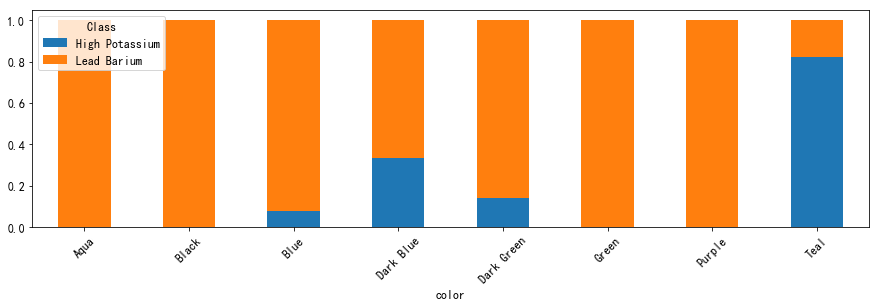
\includegraphics[width=0.95\textwidth]{15.png} 
	\caption{术后满意度与特征的定量联系} 
	\label{Fig.main15} 
\end{figure}
                       
这也进一步对分类的指标有了具体化的体现,说明上面的简单的相关性分析往往只能摸索出浅层次的结论,本文选用的随机森林算法具有深度挖掘类别与特征之间联系的能力,且具有推广价值。




















% ------------------------------------------------------------ %
%    打开chapter文件夹里的模型评价.tex文件,编辑其中的内容
% ------------------------------------------------------------ %
%    打开chapter文件夹里的模型评价.tex文件,编辑其中的内容
% ------------------------------------------------------------ %
\section{模型评价和改进}

\subsection{模型优点}

\begin{enumerate}
  \item 本文使用特征编码将数据集中的类别特征巧妙转化为数值特征,便于分析特征,以便提高模型的精度。
  \item 本文充分考虑到变量与变量之间的相关性,使用主成分分析法对原有的数据进行降维,可以使得特征的选择更加客观。
  \item 在问题三中通过施加噪音对模型的灵敏度进行分析,可以使得模型评价更为客观。
  \item 对于回归任务利用线性加权的得到更加精确的回归模型,极大的提高了模型的精度和科学性。
  \item 对于问题四不仅找到与术后满意度关联的因素,还进一步利用随机森林挖掘出了关联因素的分类规则。
\end{enumerate}




\subsection{基于Voting的模型推广}

对于问题一中的分类任务,本文考虑模型的数学可解释性,同时鉴于经过上采样和适当的数据预处理、特征工程处理后的二分类问题应当有优异的性能,未使用一些复杂的机器学习算法,取而代之的是兼具较好性能和数学可解释性的K最近邻算法。然而题设背景为临床医学,这无疑要求本文提供一个尽可能最优的不良反应预判模型——尽管这个模型数学可解释性可能不强。

对于分类任务来说,学习器从类别标记集合中预测出一个标记,最常见的组合策略是使用投票法,记学习器${{h}_{i}}$在样本$\overrightarrow{x}$上预测输出为一个$N$维向量:

\begin{equation}
    \left( h_{i}^{1}\left( \overrightarrow{x} \right),h_{i}^{2}\left( \overrightarrow{x} \right),\cdots ,h_{i}^{N}\left( \overrightarrow{x} \right) \right).
\end{equation}
其中$h_{i}^{j}\left( \overrightarrow{x} \right)$是${{h}_{i}}$在类别标记上的输出。

\begin{figure}[H] % 这个H不要动!
	\centering % 不要动!
	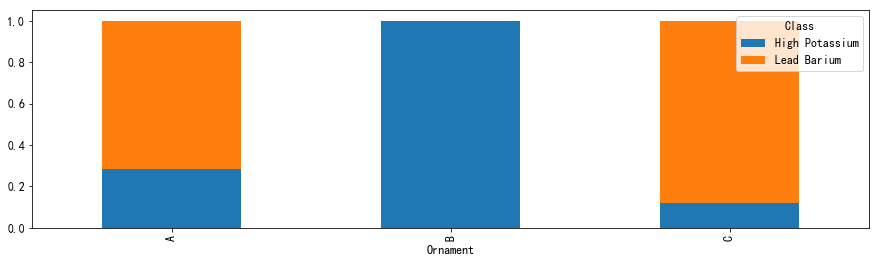
\includegraphics[width=0.95\textwidth]{14.png} 
	\caption{Voting原理图} 
	\label{Fig.main14} 
\end{figure}


对于分类模型,本文欲基于模型融合算法VotingClassifier将多个性能优良的基分类器融合在一起。下文中的分析与评价均以“呛咳”为标签的分类任务为例。本文选取7个经典的分类模型,经过训练集训练后在测试集上测试,以Accuracy\_score为初步的评价指标,结果如下:

\begin{table}[H]
    \centering  
    \caption{分类器泛化能力评价——以Accuracy\_score为指标}
    \begin{tabular}{c c c}  
    	\toprule[1.5pt]  
    	分类器        & Accuracy\_score \\  
    	\midrule[1pt]    
    	逻辑回归      & 0.646 \\ 
    	线性判别分析  & 0.63941 \\ 
    	K最近邻       &  0.90985 \\ 
    	决策树        & 0.97694 \\ 
    	朴素贝叶斯    &  0.61635 \\ 
    	支持向量机    & 0.66247 \\ 
    	XGBoost       &  0.97904 \\ 
    	\toprule[1.5pt]  
    \end{tabular}  
\end{table} 

基于上面的初步测试,本文选择决策树、K最近邻、XGBoost、Catboost作为基分类器,通过Voting中的软投票对四个分类器进行融合,结果如下:

\begin{table}[H]
    \centering  
    \caption{Voting与基分类器性能对比}
    \begin{tabular}{c c c}  
    	\toprule[1.5pt]  
    	分类器        & Accuracy\_score \\  
    	\midrule[1pt]    
    	XGB & 0.97904 \\
        KNN & 0.90985 \\
        DT  & 0.97694 \\
        Voting & 0.98113 \\
    	\toprule[1.5pt]  
    \end{tabular}  
\end{table} 

进一步地,为了更直观地展示Voting的泛化能力,本文通过混淆矩阵和ROC图对Voting的性能进行可视化:

\begin{figure}[H] % 这个H不要动!
	\centering % 不要动!
	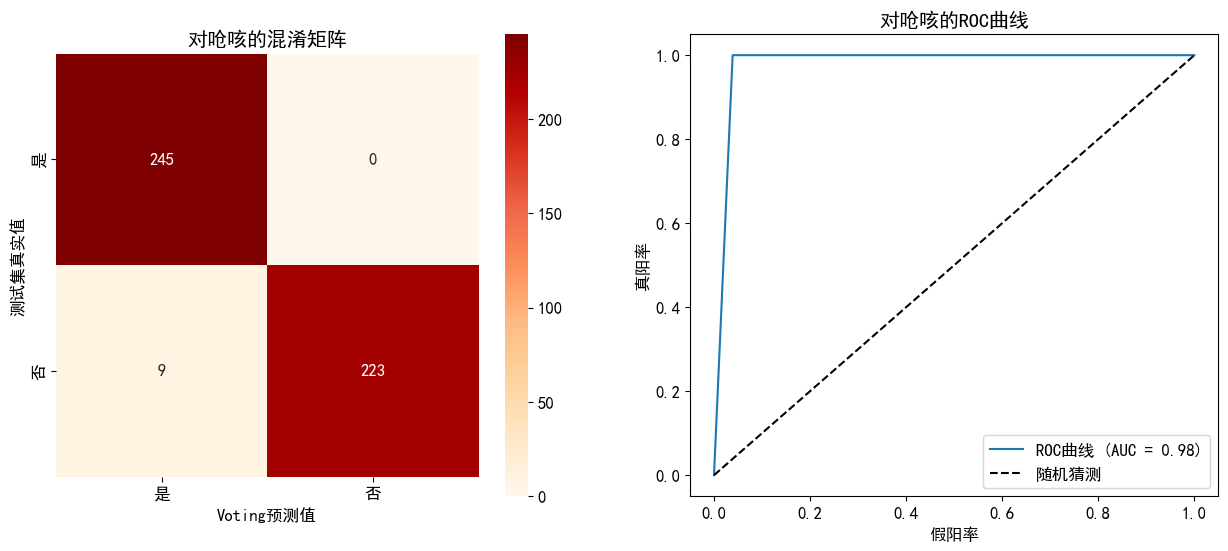
\includegraphics[width=0.95\textwidth]{13.png} 
	\caption{Voting的混淆矩阵与ROC图} 
	\label{Fig.main13} 
\end{figure}

可以见得Voting的分类性能要比KNN更好,将其应用在临床医学中才更符合人工智能服务人类的初衷。
















% ------------------------------------------------------------ %
%    打开chapter文件夹里的参考文献.tex文件,编辑其中的内容
% ------------------------------------------------------------ %
%    打开chapter文件夹里的参考文献.tex文件,编辑其中的内容
% ------------------------------------------------------------ %
\section{参考文献}


% -------改下面的参考文献内容就行,别动这两句话!!!------- %
\renewcommand{\refname}{}
\vspace{-3em}  
% -------改下面的参考文献内容就行,别动这两句话!!!------- %


\begin{thebibliography}{200}  
	\bibitem{ref1}郭躬德,黄杰,陈黎飞. 基于KNN模型的增量学习算法[J]. 模式识别与人工智能,2010,23(05):701-707.
	\bibitem{ref2}申晴,张连增. 一种新的银行信用风险识别方法:SVM-KNN组合模型[J]. 金融监管研究,2020,(07):23-37.
	\bibitem{ref3}Benarafa Halima,Benkhalifa Mohammed,Akhloufi Moulay. WordNet Semantic Relations Based Enhancement of KNN Model for Implicit Aspect Identification in Sentiment Analysis[J]. International Journal of Computational Intelligence Systems,2023,16(1).
	\bibitem{ref4}王大鹏, 闫肃, 王楠, 等. 基于卡方检验和秩和检验的智慧消防行业分析[J]. 消防科学与技术, 2022, 41(11): 1594.
	\bibitem{ref5}王皓辰, 张长伦, 黎铭亮. 基于深度学习的点云上采样算法研究[J]. Journal of Image and Signal Processing, 2023, 12: 21.
	\bibitem{ref6}梁胜杰,张志华,崔立林. 主成分分析法与核主成分分析法在机械噪声数据降维中的应用比较[J]. 中国机械工程,2011,22(01):80-83.
	\bibitem{ref7}曹前. 基于二阶多项式回归和权重主成分分析法的多光谱降维算法研究[J]. Optical Technique, 2023, 49(2): 250-256.
	\bibitem{ref8}Wan Minghua,Wang Xichen,Tan Hai,Yang Guowei. Manifold Regularized Principal Component Analysis Method Using L2,p-Norm[J]. Mathematics,2022,10(23).
    \bibitem{ref9}张凯, 张科. 基于 LightGBM 算法的边坡稳定性预测研究[J]. 中国安全科学学报, 2022, 32(7): 113.
    \bibitem{ref10}Yang Qiang,Feng Yan,Guan Li,Wu Wenyu,Wang Sichen,Li Qiangyu. X-Band Radar Attenuation Correction Method Based on LightGBM Algorithm[J]. Remote Sensing,2023,15(3).
    \bibitem{ref11}Anand L.,Mewada Shivlal,Shamsi WameedDeyah,Ritonga Mahyudin,Aflisia Noza,KumarSarangi Prakash,NdoleArthur Moses. Diagnosis of Prostate Cancer Using GLCM Enabled KNN Technique by Analyzing MRI Images[J]. BioMed Research International,2023,2023.
    \bibitem{ref12}张晓辉, 李莹, 王华勇, 等. 应用特征聚合进行中文文本分类的改进 KNN 算法[J]. 东北大学学报: 自然科学版, 2003, 24(3): 229-232.
    \bibitem{ref13}Roshanfekr Behnam,Amirmazlaghani Maryam,Rahmati Mohammad. Learning graph from graph signals: An approach based on sensitivity analysis over a deep learning framework[J]. Knowledge-Based Systems,2023,260.
    \bibitem{ref14}彭高辉, 王志良. 数据挖掘中的数据预处理方法[J]. 华北水利水电学院学报, 2008 (6): 61-63.
    \bibitem{ref15}ParedesSalazar Enrique A,CalderónCárdenas Alfredo,Varela Hamilton. Sensitivity Analysis in the Microkinetic Description of Electrocatalytic Reactions.[J]. The journal of physical chemistry. A,2022,126(17).
    \bibitem{ref16}吴庶宸, 戚宗锋, 李建勋. 基于深度学习的智能全局灵敏度分析[J]. 上海交通大学学报, 2022, 56(7): 840.
    \bibitem{ref17}任家东,刘新倩,王倩,何海涛,赵小林. 基于KNN离群点检测和随机森林的多层入侵检测方法[J]. 计算机研究与发展,2019,56(03):566-575.
    \bibitem{ref18}Li Zhenglei,Chen Yu,Tao Yan,Zhao Xiuge,Wang Danlu,Wei Tong,Hou Yaxuan,Xu Xiaojing. Mapping the personal PM2.5 exposure of China's population using random forest[J]. Science of the Total Environment,2023,871.
    \bibitem{ref19}张著英,黄玉龙,王翰虎. 一个高效的KNN分类算法[J]. 计算机科学,2008,(03):170-172.
    \bibitem{ref20}方匡南,吴见彬,朱建平,谢邦昌. 随机森林方法研究综述[J]. 统计与信息论坛,2011,26(03):32-38.
\end{thebibliography} 
\newpage



% ------------------------------------------------------------ %
%    打开chapter文件夹里的附录.tex文件,编辑其中的内容
% ------------------------------------------------------------ %
%    打开chapter文件夹里的附录.tex文件,编辑其中的内容
% ------------------------------------------------------------ %
% -----------------------------------------------------
% 下面的附录格式仅供参考,说不定大家到时候时间太紧都
% 没时间写附录了,附录这部分是最开放的哈,想怎么写怎
% 么写,主要内容就是代码和你想放在文章里又没放的东西,
% 比如大型图表等。
% -----------------------------------------------------

\appendix  % 别动!!!

\section{附录:本文全部解答过程的流程图}

\subsection{第一题流程图}

\begin{figure}[H] % 这个H不要动!
	\centering % 不要动!
	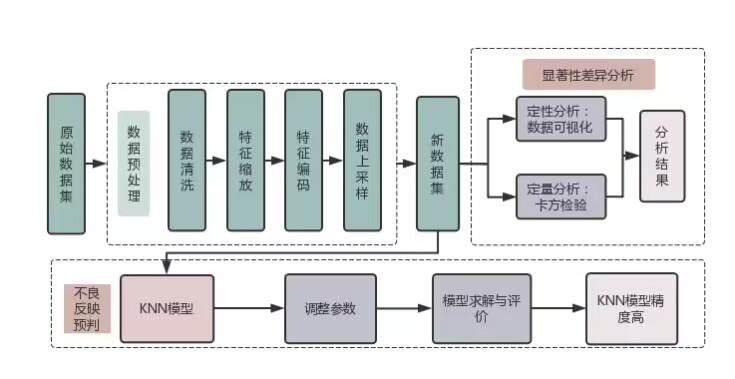
\includegraphics[width=0.95\textwidth]{流程图1.png} 
	\caption{问题一全过程流程图} 
	\label{Fig.main10001} 
\end{figure}

\subsection{第二题流程图}

\begin{figure}[H] % 这个H不要动!
	\centering % 不要动!
	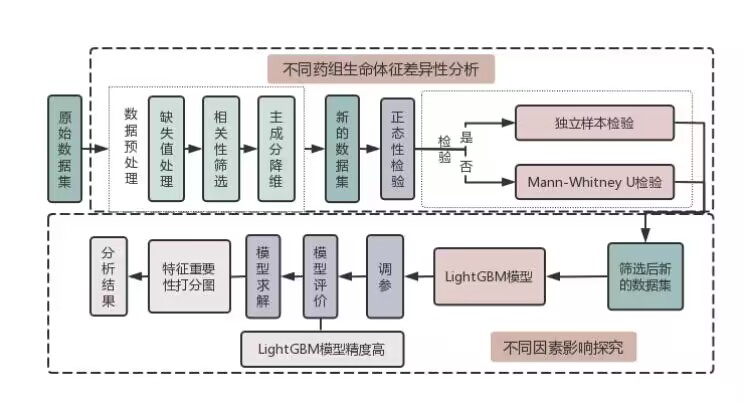
\includegraphics[width=0.95\textwidth]{流程图2.png} 
	\caption{问题二全过程流程图} 
	\label{Fig.main10002} 
\end{figure}

\subsection{第三题流程图}

\begin{figure}[H] % 这个H不要动!
	\centering % 不要动!
	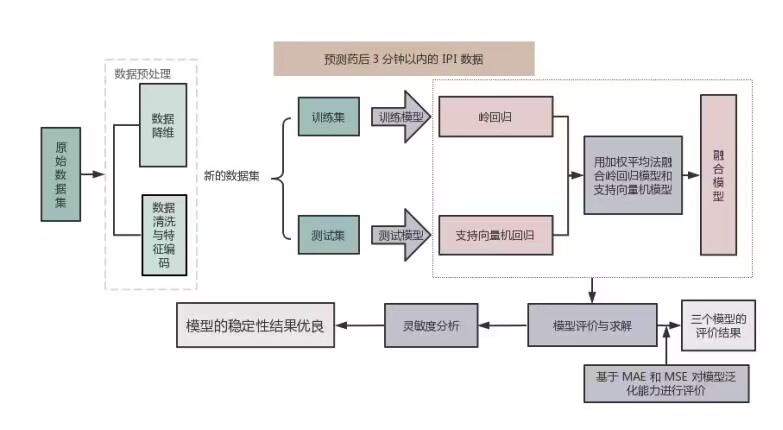
\includegraphics[width=0.95\textwidth]{流程图3.png} 
	\caption{问题三全过程流程图} 
	\label{Fig.main10003} 
\end{figure}

\subsection{第四题流程图}

\begin{figure}[H] % 这个H不要动!
	\centering % 不要动!
	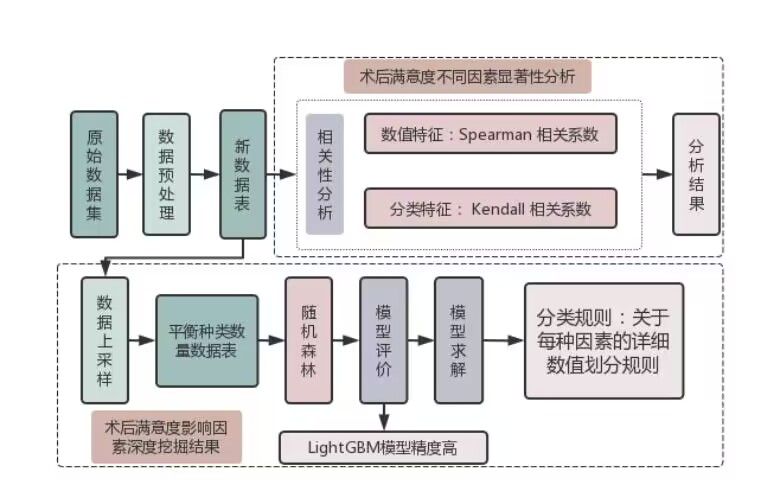
\includegraphics[width=0.95\textwidth]{流程图4.png} 
	\caption{问题四全过程流程图} 
	\label{Fig.main10004} 
\end{figure}

\section{附录:图表}

\subsection{完整KNN测试的混淆矩阵、ROC图}

\begin{figure}[H] % 这个H不要动!
	\centering % 不要动!
	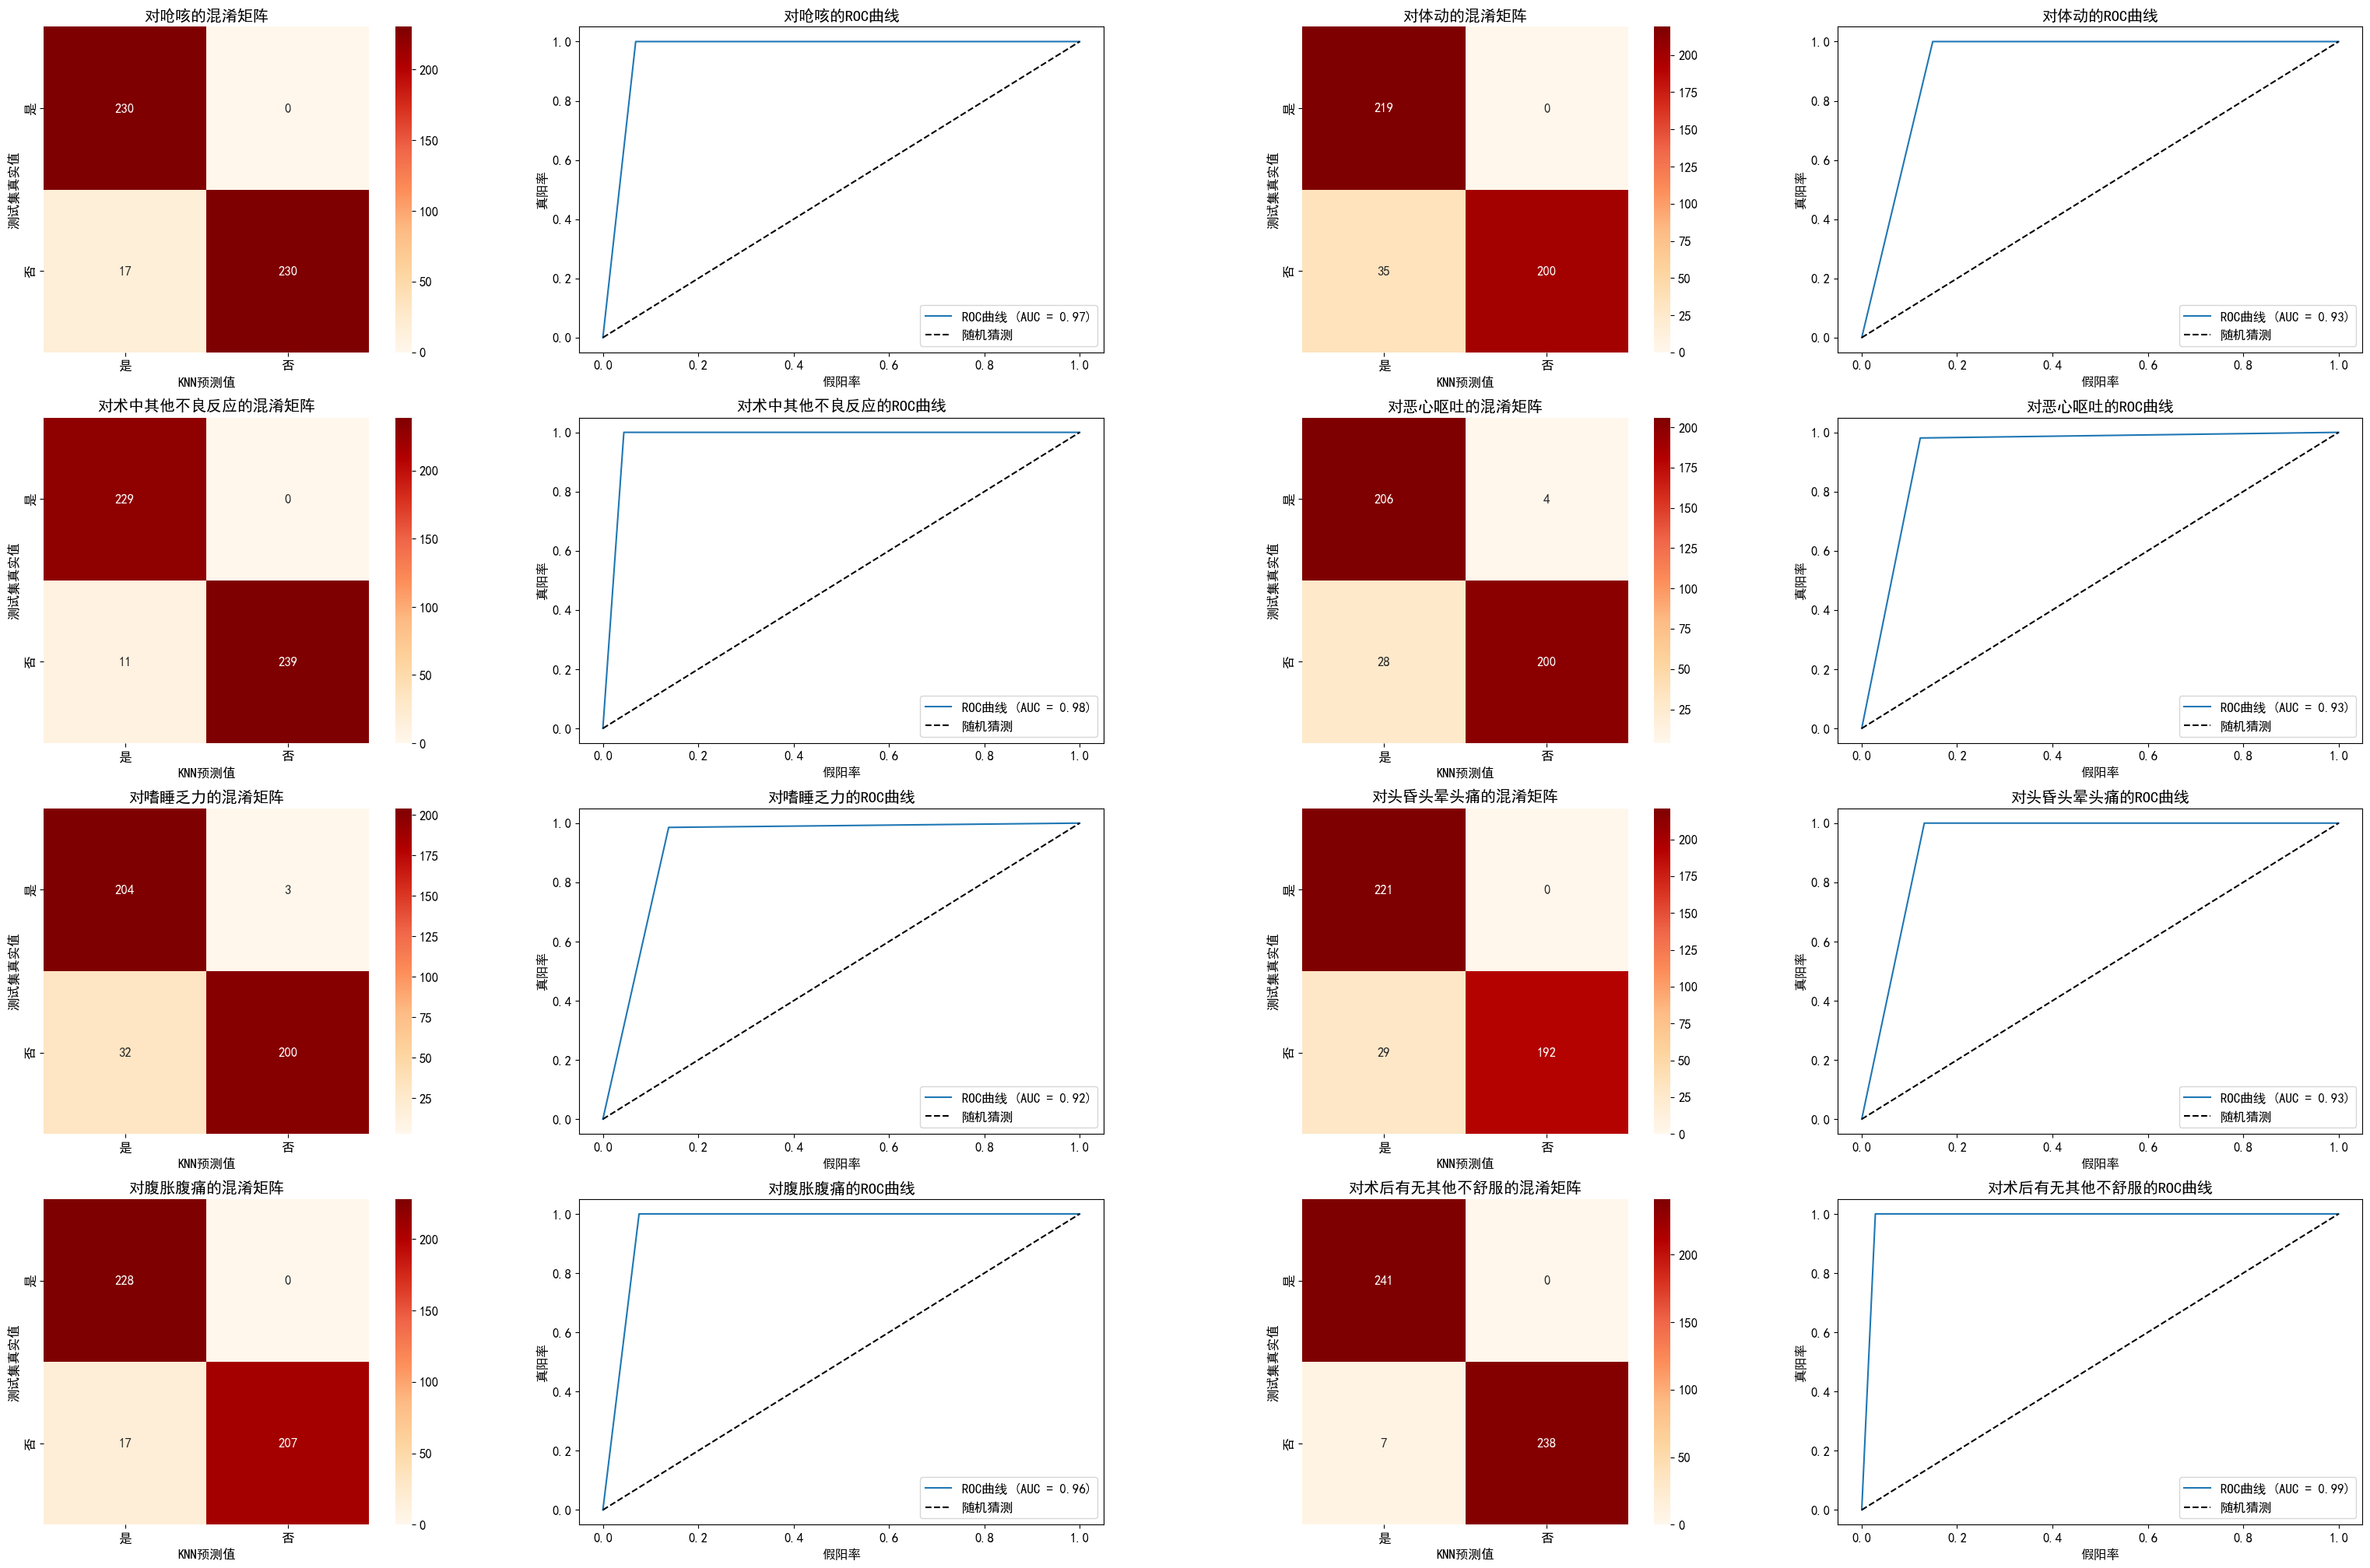
\includegraphics[width=0.95\textwidth]{附录1.png} 
	\caption{完整KNN测试结果的混淆矩阵和ROC图} 
	\label{Fig.main10005} 
\end{figure}

\subsection{六次回归的灵敏度分析图}

\begin{figure}[H] % 这个H不要动!
	\centering % 不要动!
	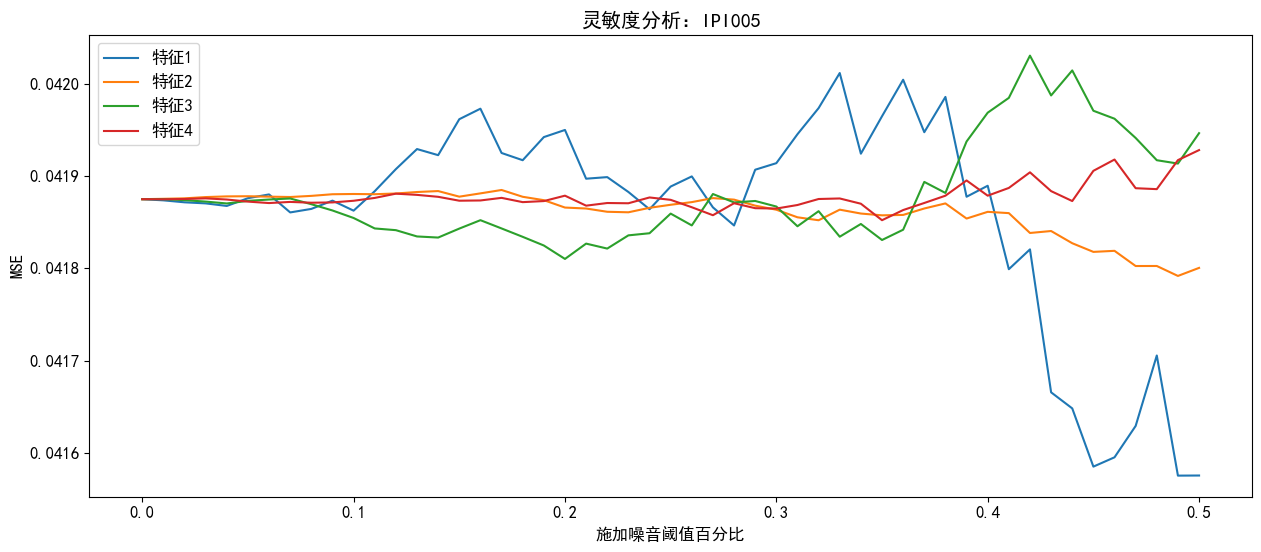
\includegraphics[width=0.95\textwidth]{附录2-1.png} 
	\label{Fig.main10016} 
\end{figure}

\begin{figure}[H] % 这个H不要动!
	\centering % 不要动!
	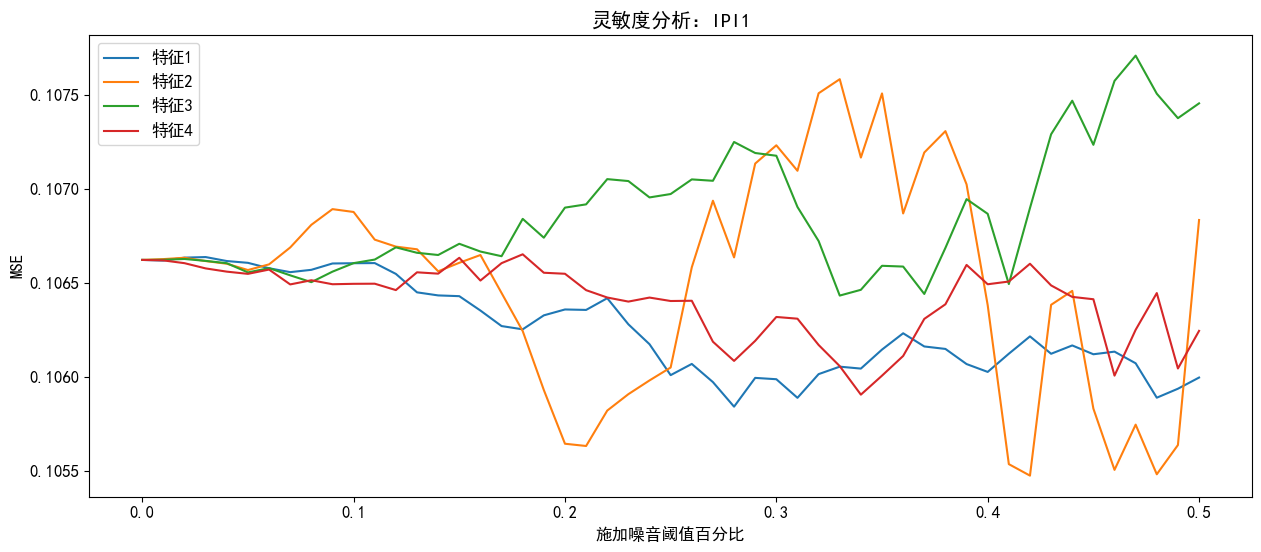
\includegraphics[width=0.95\textwidth]{附录2-2.png} 
	\label{Fig.main1002} 
\end{figure}

\begin{figure}[H] % 这个H不要动!
	\centering % 不要动!
	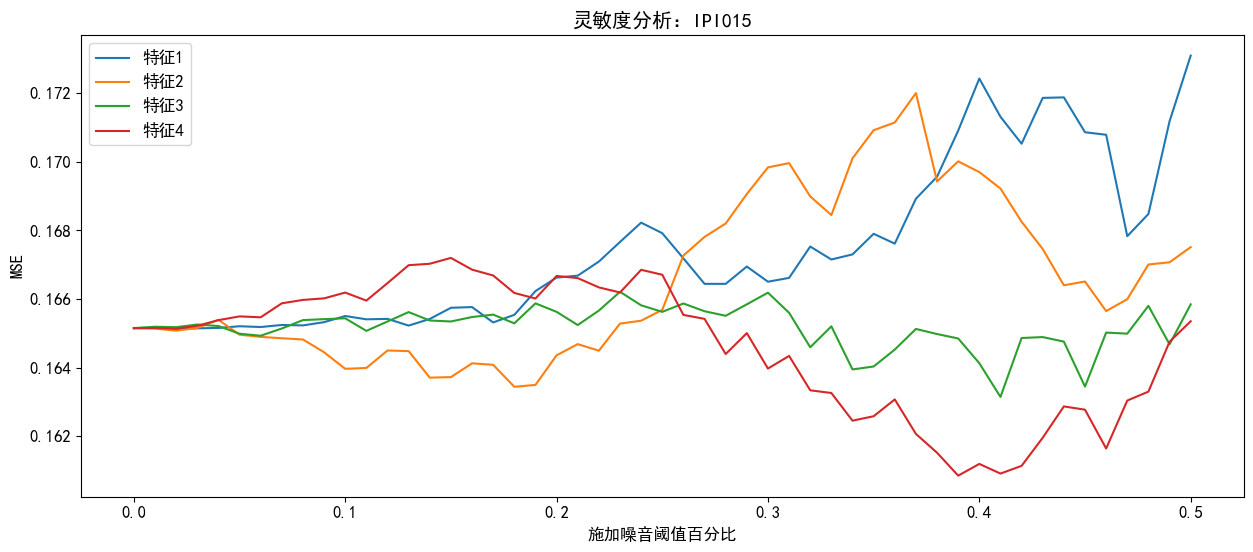
\includegraphics[width=0.95\textwidth]{附录2-3.png} 
	\label{Fig.main1003} 
\end{figure}

\begin{figure}[H] % 这个H不要动!
	\centering % 不要动!
	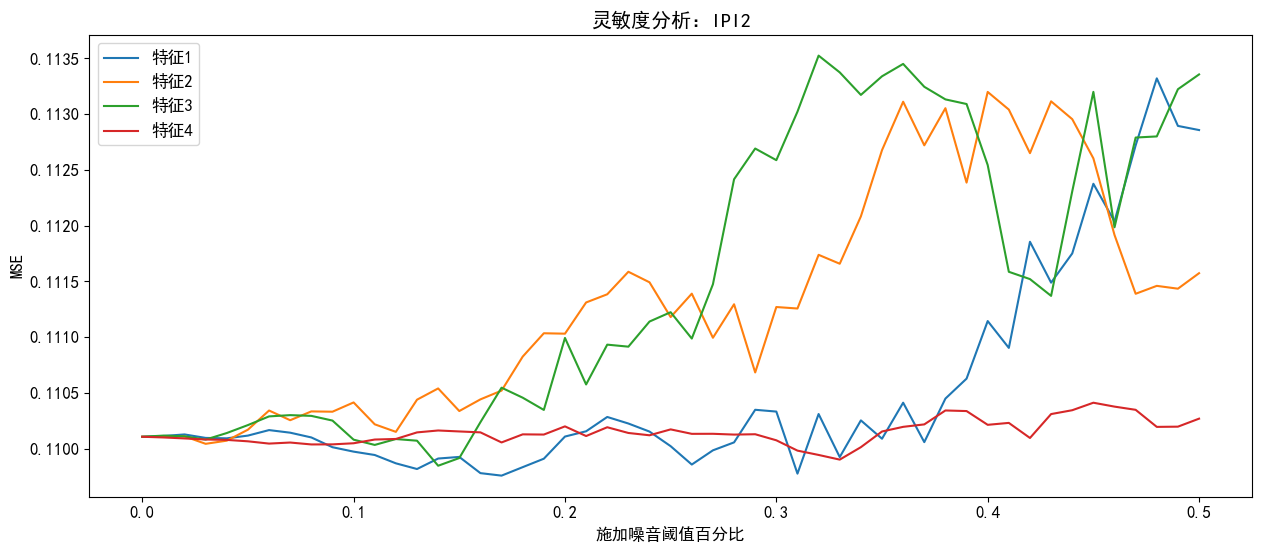
\includegraphics[width=0.95\textwidth]{附录2-4.png} 
	\label{Fig.main1004} 
\end{figure}

\begin{figure}[H] % 这个H不要动!
	\centering % 不要动!
	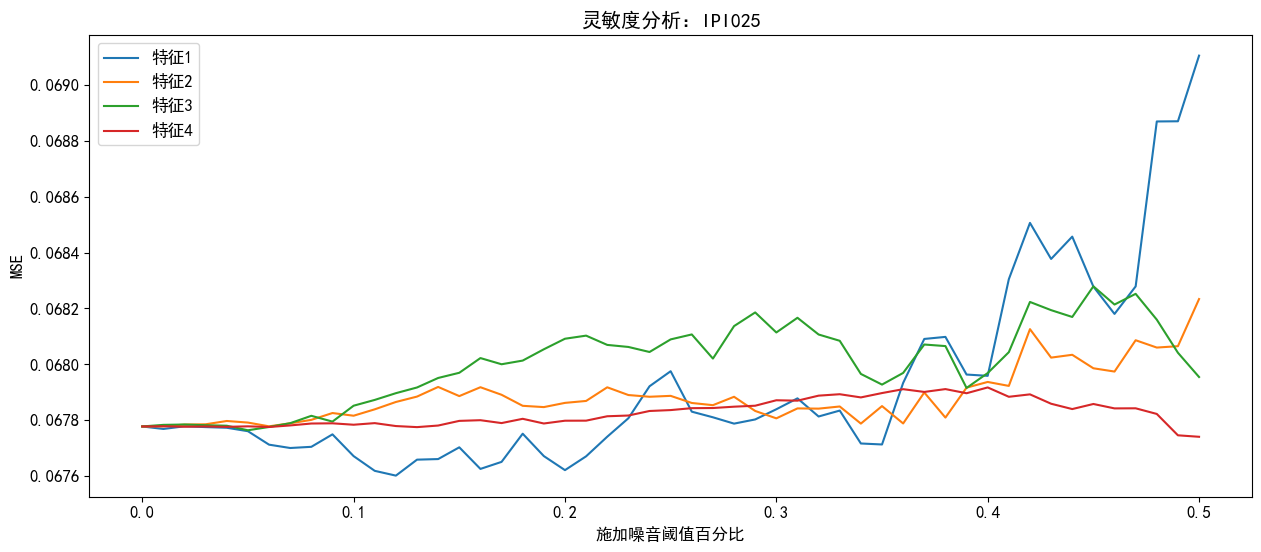
\includegraphics[width=0.95\textwidth]{附录2-5.png} 
	\label{Fig.main1005} 
\end{figure}

\begin{figure}[H] % 这个H不要动!
	\centering % 不要动!
	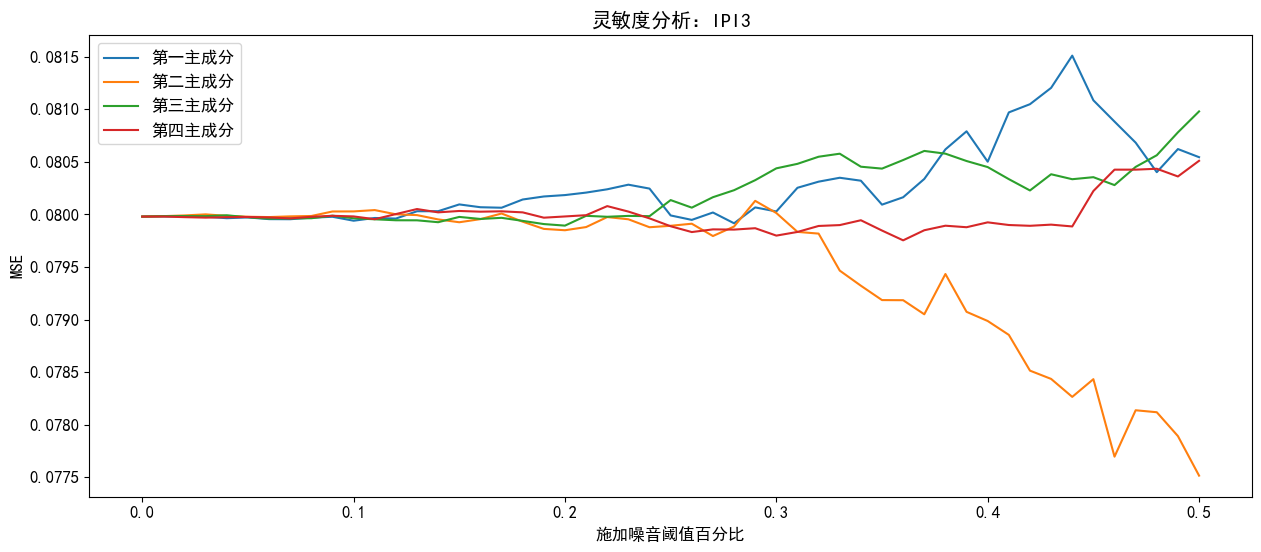
\includegraphics[width=0.95\textwidth]{附录2-6.png} 
	\label{Fig.main1006} 
\end{figure} 


\section{附录:代码}

附录代码仅为重要功能实现部分,完整代码参照提交的附件,附件内代码均为ipynb(Jupyter Notebook),路径均为相对路径,可以直接运行。

\subsection{卡方检验}

\begin{lstlisting}[language=Python]
# 创建一个交叉表格,以Sex和Category作为行列索引
cross_table = pd.crosstab(df1['镇静药名称'], df1['呛咳'])

# 进行卡方检验,并返回卡方值、p值、自由度和期望值等相关信息
chi2, p_value, dof, expected = stats.chi2_contingency(cross_table)

# 输出检验结果
# print(f"卡方值: {chi2}")
# print(f"p值: {p_value}")
# print(f"自由度: {dof}")
# print(f"期望值: \n{expected}")

if p_value < 0.05:
    print('关于呛咳,两种药有显著差异')
else:
    print('关于呛咳,两种药没有显著差异')
\end{lstlisting}

\subsection{KNN模型建立与评价}

\begin{lstlisting}[language=Python]
# ----------------------------------------------
#                     模型准备
# ----------------------------------------------
# 特征空间:独热编码
X = pd.get_dummies(df2[['性别','年龄','身高','体重','有无手术史','有无既往史',
          '是否吸烟','是否酗酒','镇静药名称']])

# 数据归一化
model = MinMaxScaler()
X[['年龄','身高','体重']] = model.fit_transform(df2[['年龄','身高','体重']])

# 字符串换成数字
df2["呛咳"] = df2["呛咳"].map({"有": 1, "无": 0})
df2["体动"] = df2["体动"].map({"有": 1, "无": 0})
df2["术中其他"] = df2["术中其他"].map({"有": 1, "无": 0})
df2["是否恶心呕吐"] = df2["是否恶心呕吐"].map({"是": 1, "否": 0})
df2["是否头晕头昏头痛"] = df2["是否头晕头昏头痛"].map({"是": 1, "否": 0})
df2["是否嗜睡乏力"] = df2["是否嗜睡乏力"].map({"是": 1, "否": 0})
df2["是否腹胀腹痛"] = df2["是否腹胀腹痛"].map({"是": 1, "否": 0})
df2["有无其他不舒服"] = df2["有无其他不舒服"].map({"是": 1, "否": 0})



# ----------------------------------------------
#                   上采样
# ----------------------------------------------
# 创建上采样对象
ros = RandomOverSampler(random_state=42)
# 对数据进行上采样
X_resampled, y_resampled = ros.fit_resample(X, df2.呛咳)

# 定义参数搜索空间
param_grid = {
    'n_neighbors': np.arange(1, 11),
    'weights': ['uniform', 'distance'],
    'algorithm': ['auto', 'ball_tree', 'kd_tree', 'brute'],
    'leaf_size': np.arange(10, 51, 10),
    'p': [1, 2, 3]
}

# ----------------------------------------------
#               GridSearchCV调参
# ----------------------------------------------
# 初始化KNN模型
knn = KNeighborsClassifier()

# 使用网格搜索进行调参
grid_search = GridSearchCV(knn, param_grid=param_grid, cv=5)
grid_search.fit(X_resampled, y_resampled)

# 输出最佳参数和最佳得分
print("Best parameters: {}".format(grid_search.best_params_))
print("Best cross-validation score: {:.2f}".format(grid_search.best_score_))

# ----------------------------------------------
#           以“呛咳”为例的KNN预测实现
# ----------------------------------------------
# 创建上采样对象
ros = RandomOverSampler(random_state=42)
# 对数据进行上采样
X_resampled, y_resampled = ros.fit_resample(X, df2.呛咳)

# 划分数据集
X1_train, X1_test, y1_train, y1_test = train_test_split(X_resampled, y_resampled, test_size=0.2, random_state=0)

Model = KNeighborsClassifier(algorithm='auto', leaf_size=10, 
                            n_neighbors=1, p=3, weights='uniform')
y1_pred = Model.fit(X1_train, y1_train).predict(X1_test)

# 模型评价
print("评估数据结果打印:\n", classification_report(y1_test, y1_pred))

# ----------------------------------------------
#             混淆矩阵与ROC曲线
# ----------------------------------------------
mat1 = confusion_matrix(y1_test, y1_pred, 
                labels=[1, 0])
fpr1, tpr1, thresholds1 = roc_curve(y1_test, y1_pred)
auc1 = roc_auc_score(y1_test, y1_pred)

plt.subplot(1, 2, 1)
sns.heatmap(mat1, annot=True, square="equal", cmap="OrRd", fmt="d",
    xticklabels=["是", "否"], 
    yticklabels=["是", "否"])
plt.xlabel("KNN预测值")
plt.ylabel("测试集真实值")
plt.title("对呛咳的混淆矩阵")

plt.subplot(1, 2, 2)
# 绘制ROC曲线和y=x的对角线
plt.plot(fpr1, tpr1, label='ROC曲线 (AUC = {:.2f})'.format(auc1))
plt.plot([0, 1], [0, 1], 'k--', label='随机猜测')
plt.xlabel('假阳率')
plt.ylabel('真阳率')
plt.title('对呛咳的ROC曲线')
plt.legend()
\end{lstlisting}


\subsection{主成分分析法}

\begin{lstlisting}[language=Python]
# ----------------------------------------------
#   先试探,用可视化图确定具体降维多少
# ----------------------------------------------
# 创建PCA对象并进行降维
pca = PCA(n_components=49)
df_try = pca.fit_transform(df3[['sbp00', 'dbp00', 'petco200', 'RR00', 'spo200', 'HR00', 'IPI00', 'moaas00',
    'petco2005','RR005','spo2005','HR005','IPI005','moaas005','sbp1','dbp1',
    'petco21','RR1','spo21','HR1','IPI1','moaas1','sbpjinjing','dbpjinjing','petco2jinjing',
    'RRjinjing','spo2jinjing','HRjinjing','IPIjinjing','moaasjinjing','petco2015',
    'RR015','spo2015','HR015','IPI015','moaas015','sbp2','dbp2','petco22','RR2','spo22',
    'HR2','IPI2','moaas2','petco2025','RR025','spo2025','HR025','IPI025',
    'moaas025','sbp3','dbp3','petco23','RR3','spo23','HR3','IPI3','moaas3','sbp5',
    'dbp5','petco25','RR5','spo25','HR5','IPI5','moaas5','sbp7','dbp7','petco27',
    'RR7','spo27','HR7','IPI7','moaas7','sbpjieshu',
    'dbpjieshu','petco2jieshu','RRjieshu','spo2jieshu','HRjieshu','IPIjieshu']])

# 绘制主成分方差解释比例图
plt.figure(figsize=(20, 5))
plt.plot(np.cumsum(pca.explained_variance_ratio_))
plt.xlabel('降维所得个数')
plt.ylabel('主成分的方差解释比例')
plt.title('主成分的方差解释比例图')
plt.show()

# ----------------------------------------------
#   主成分分析法实现数据降维
# ----------------------------------------------
# 创建PCA对象并进行降维
pca = PCA(n_components=10)
df4 = pd.DataFrame(pca.fit_transform(df3.drop(['镇静药名称','性别','年龄','身高',
                                            '体重','有无手术史','有无既往史','是否吸烟',
                                            '是否酗酒','有无PONV','有无晕动史'], axis=1)))
\end{lstlisting}


\subsection{独立样本检验}

\begin{lstlisting}[language=Python]
# ----------------------------------------------
#             进行正态性检验
# ----------------------------------------------
stat, p = normaltest(df[1])
if p < 0.05:
    print('参数检验')
else:
    print('非参数检验')
    
# ----------------------------------------------
#                   独立样本t检验
# ----------------------------------------------
# 将标签数据根据性别分成两组
e1 = df.loc[df['镇静药组'] == 1, 'label1']
e2 = df.loc[df['镇静药组'] == 0, 'label1']

# 进行独立样本t检验
fvalue, pvalue = ttest_ind(e1, e2)

# 输出结果
print("F值为:", fvalue)
print("p值为:", pvalue)

# ----------------------------------------------
#               Mann-Whitney U
# ----------------------------------------------
# 将标签数据根据性别分成两组
e1 = df.loc[df['镇静药组'] == 1, 'label2']
e2 = df.loc[df['镇静药组'] == 0, 'label2']

# 进行Mann-Whitney U检验
fvalue, pvalue = mannwhitneyu(e1, e2)

# 输出结果
print("F值为:", fvalue)
print("p值为:", pvalue)

\end{lstlisting}

\subsection{LightGBM建模与特征重要性分析}

\begin{lstlisting}[language=Python]
# ----------------------------------------------
#               划分数据集
# ----------------------------------------------
X1_train, X1_test, y1_train, y1_test = train_test_split(X, df[3], train_size=0.8, random_state=1)


# ----------------------------------------------
#              GridSearchCV调参
# ----------------------------------------------
model = lgb.LGBMRegressor(learning_rate=0.1)
param = {
        "max_depth":[4, 7, 10],
        "num_leaves":[300, 600, 900],
        "n_estimators":[10, 70, 130],
        'min_child_samples': [18, 20, 22],
        'min_child_weight':[0.001, 0.002]
        }

grid_search3 = GridSearchCV(model, n_jobs=-1, param_grid=param, cv=5, scoring="neg_mean_squared_error")
grid_search3.fit(X1_train, y1_train)
grid_search3.best_estimator_, grid_search3.best_score_

X1_train, X1_test, y1_train, y1_test = train_test_split(X, df[3], train_size=0.8, random_state=1)


# ----------------------------------------------
#            LightGBM模型建立
# ----------------------------------------------
model1 = lgb.LGBMRegressor(max_depth=7, min_child_samples=22, n_estimators=10,num_leaves=300)
y1_pred = model1.fit(X1_train, y1_train).predict(X1_test)


# ----------------------------------------------
#            LightGBM模型评价
# ----------------------------------------------
# Mean Absolute Error(平均绝对误差)
print(mean_absolute_error(y1_test, y1_pred))

# Mean Squared Error(均方误差)
print(mean_squared_error(y1_test, y1_pred))

names = ['镇静药名称','性别','年龄','身高','体重','有无手术史','有无既往史',  
        '是否吸烟','是否酗酒','有无PONV','有无晕动史']

# ----------------------------------------------
#            LightGBM特征重要性打分
# ----------------------------------------------
plt.figure(figsize=(15, 5))
plt.title("生命体征第三主成分的影响探究")
plt.xlabel("可能的影响因素")
plt.ylabel("特征重要性打分")
plt.bar(names, model1.feature_importances_, color='b')
plt.show()
\end{lstlisting}

\subsection{回归器的模型融合与灵敏度分析}

\begin{lstlisting}[language=Python]
# ----------------------------------------------
#            岭回归的实现
# ----------------------------------------------
# 模型初始化
ridge = Ridge(alpha=1)
# 模型训练、模型预测
y1_pred1 = ridge.fit(X1_train, y1_train).predict(X1_test)
# Mean Squared Error(均方误差)
MSE_1 = mean_squared_error(y1_test, y1_pred1)
# Mean Absolute Error(平均绝对误差)
MAE_1 = mean_absolute_error(y1_test, y1_pred1)

print(MSE_1)
print(MAE_1)

# ----------------------------------------------
#            支持向量机的实现
# ----------------------------------------------
# 支持向量机
svr = SVR(kernel='rbf')
# 模型训练、模型预测
y1_pred2 = svr.fit(X1_train, y1_train).predict(X1_test)
# Mean Squared Error(均方误差)
MSE_2 = mean_squared_error(y1_test, y1_pred2)
# Mean Absolute Error(平均绝对误差)
MAE_2 = mean_absolute_error(y1_test, y1_pred2)

print(MSE_2)
print(MAE_2)

# ----------------------------------------------
#            加权平均法的实现
# ----------------------------------------------
w1 = 1 / MSE_1
w2 = 1 / MSE_2
w1_normalized = w1 / (w1 + w2)
w2_normalized = w2 / (w1 + w2)

y1_pred = w1_normalized * y1_pred1 + w2_normalized * y1_pred2

print(mean_squared_error(y1_test, y1_pred))
print(mean_absolute_error(y1_test, y1_pred))


# ----------------------------------------------
#            灵敏度分析
# ----------------------------------------------
def analysis(X1_test):
    # 接受过噪音的X_test得分情况
    score_1, score_2, score_3, score_4 = [], [], [], []

    for j in range(0, 4):

        # 备份新的X_test用于噪音处理
        df1 = np.array(X1_test.copy())
        # 打印X_test的维数,方便后面做循环
        m, n = np.array(X1_test).shape
        # 噪音
        error = np.ones(shape=(m, 1))

        # 按0到0.5的比例对X_test进行噪音处理
        for i in np.linspace(0, 0.5, 51):

            # 施加对应比例噪音并添加到X_test上,产生新的测试集特征df2
            error[:, 0] = np.random.uniform(-i * df1[:, j], i * df1[:, j])
            df1[:, j] = df1[:, j] + error[:, 0]
            df2 = pd.DataFrame(df1)
            df2.columns = ['特征1', '特征2', '特征3', '特征4']

            # 构建完数据后预测、打分
            y_pred1 = pd.DataFrame(ridge.predict(df2))
            y_pred2 = pd.DataFrame(svr.predict(df2))
            MSE_1 = mean_squared_error(y1_test, y_pred1)
            MSE_2 = mean_squared_error(y1_test, y_pred2)

            w1 = 1 / MSE_1
            w2 = 1 / MSE_2
            w1_normalized = w1 / (w1 + w2)
            w2_normalized = w2 / (w1 + w2)

            y_pred = w1_normalized * y_pred1 + w2_normalized * y_pred2
        
            if j == 0:
                score_1.append(mean_squared_error(y1_test, y_pred))
            elif j == 1:
                score_2.append(mean_squared_error(y1_test, y_pred))
            elif j == 2:
                score_3.append(mean_squared_error(y1_test, y_pred))
            else:
                score_4.append(mean_squared_error(y1_test, y_pred))
    
    return score_1, score_2, score_3, score_4

score_1, score_2, score_3, score_4 = analysis(X1_test)

plt.figure(figsize=(15, 6))
plt.rcParams["font.sans-serif"] = ["SimHei"]
plt.rcParams['font.size'] = 12  # 字体大小
plt.rcParams['axes.unicode_minus'] = False  # 正常显示负号
plt.xlabel("施加噪音阈值百分比")
plt.ylabel("MSE")

plt.plot(np.linspace(0, 0.5, 51), score_1, label="特征1")
plt.plot(np.linspace(0, 0.5, 51), score_2, label="特征2")
plt.plot(np.linspace(0, 0.5, 51), score_3, label="特征3")
plt.plot(np.linspace(0, 0.5, 51), score_4, label="特征4")

plt.title("灵敏度分析:IPI005")
plt.legend()
plt.show()
\end{lstlisting}



\subsection{随机森林的建模与树状图导出}


\begin{lstlisting}[language=Python]
# ----------------------------------------------
#            模型准备
# ----------------------------------------------
X = df1.drop("rating", axis=1)
y = df1.rating


# ----------------------------------------------
#            上采样
# ----------------------------------------------
# 创建上采样对象
ros = RandomOverSampler(random_state=42)
# 对数据进行上采样
X_resampled, y_resampled = ros.fit_resample(X, y)

X_train, X_test, y_train, y_test = train_test_split(X_resampled, y_resampled, test_size=0.2, random_state=0)


# ----------------------------------------------
#            随机森林建模与评价
# ----------------------------------------------
Model = RandomForestClassifier(max_depth=3, n_estimators=1000)
y_pred = Model.fit(X_train, y_train).predict(X_test)

# 打印分类模型最好的评价系统
print("评估数据结果打印:\n", classification_report(y_test, y_pred))

# ----------------------------------------------
#            树状图导出
# ----------------------------------------------
plt.figure(figsize=(20, 10))
estimator = Model.estimators_[5]
estimator.fit(X_train, y_train)
plot_tree(estimator, filled=True, max_depth=3, feature_names=X.columns)

plt.title("随机森林分类树状图")
plt.show()
\end{lstlisting}




\end{document} 